\documentclass{book}
\usepackage[spanish,es-nolists,es-tabla, es-nodecimaldot]{babel} % Asegúrate de incluir 'es-nolists' si no quieres que babel altere las listas.


\addto{\captionsspanish}{%
	\renewcommand{\bibname}{Referencias}
}


\usepackage[DIV=14,BCOR=2mm,headinclude=true,footinclude=false]{typearea}
\usepackage{fancyhdr}
\usepackage{subcaption}
\usepackage{multirow}
\usepackage{siunitx}
\fancypagestyle{plain}{
	\fancyhf{}
	\renewcommand{\headrulewidth}{0pt}
	\fancyfoot[C]{\thepage}
}
\pagestyle{fancy}
\fancyhf{}
\fancyfoot[C]{\thepage}

\usepackage{listings}

\usepackage{hhline}
\usepackage{caption}
\captionsetup[figure]{font=small}
\usepackage[table,dvipsnames]{xcolor}
\usepackage{colortbl} % Necesario para \cellcolor
% Paquete para idioma español

% Paquete para personalizar los márgenes
\usepackage[margin=2.5cm]{geometry}
\usepackage{adjustbox}
%Estos dos paquetes son necesarios para escribir cómodamente los
% los documentos en Español, sin necesidad de utilizar secuencias
% de escape como {\'\i} para poner una "í".
\usepackage{titlesec}
\titleformat{\chapter}[display]
{\normalfont\huge\bfseries}{\chaptertitlename\ \thechapter}{20pt}{\Huge}
\titlespacing*{\chapter}{0pt}{0pt}{40pt}
%Para incluir figuras se necesitarán las macros definidas en este paquete
\usepackage{graphicx}

% Para fijar la posición de las imágenes
\usepackage{float}     
\usepackage{xcolor}
\usepackage[table]{xcolor}
%Este paquete permite incluir y resaltar URLs
\usepackage{url}
\usepackage{amsmath, amssymb, bm}
%Este paquete, cuando se usa pdflatex, formatea el documento añadiendo
% enlaces internos entre las referencias y los objetos referenciados
% (por ejemplos, figuras, tablas, referencias de la bibliografía).
\usepackage[unicode=true, pdfusetitle, bookmarks=true, bookmarksnumbered=false, bookmarksopen=false,
breaklinks=true,pdfborder={0 0 1},backref=false,colorlinks=false]{hyperref}

\usepackage{threeparttable}
\usepackage{tabularx}
\usepackage{booktabs}
\newcommand{\ra}[1]{\renewcommand{\arraystretch}{#1}}
% Paquete para personalizar las listas
\usepackage{enumitem} 
\setlist[itemize]{label=-}

%Este paquete puede ser útil si se quieren incluir algunos símbolos
% especiales en las ecuaciones

\usepackage{array}
\usepackage{gensymb}
%Esta definición permite introducir la dirección de los autores
% y mostrarla convenientemente
\newcommand{\address}[1]{\par {\raggedright #1\vspace{1.4em}\noindent\par}}


%Inicio del documento (hasta que se cierre con \end{document}
% Paquete para personalizar los títulos de las secciones
\usepackage{titlesec}
% Paquete para modificar el formato del abstract
\usepackage{abstract}
% Modificar el formato del abstract
\renewcommand{\abstractnamefont}{\normalfont\large\bfseries}
\renewcommand{\abstracttextfont}{\normalfont\normalsize}
\newcolumntype{C}[1]{>{\centering\arraybackslash}p{#1}}
\renewenvironment{abstract}{
\begin{center}
	\bfseries\abstractname\vspace{-\baselineskip}
\end{center}
\list{}{\leftmargin1.5cm \rightmargin\leftmargin}
\item\relax
}{
\endlist
}



% Paquete para ajustar la tabla de contenidos con etoc
\usepackage{etoc}

% Estilo de artículo para cada capítulo
\titleformat{\chapter}[display]{\normalfont\huge\bfseries}{\chaptertitlename\ \thechapter}{20pt}{\Huge}


\makeatletter
\renewenvironment{thebibliography}[1]
{% Utilizamos \section{Referencias} para que aparezca numerado como una sección normal
	\section{Referencias}
	\list{\@biblabel{\@arabic\c@enumiv}}%
	{\settowidth\labelwidth{\@biblabel{#1}}%
		\leftmargin\labelwidth
		\advance\leftmargin\labelsep
		\@openbib@code
		\usecounter{enumiv}%
		\let\p@enumiv\@empty
		\renewcommand\theenumiv{\@arabic\c@enumiv}}%
	\sloppy
	\clubpenalty4000
	\@clubpenalty \clubpenalty
	\widowpenalty4000%
	\sfcode`\.\@m}
{\def\@noitemerr
	{\@latex@warning{Empty `thebibliography' environment}}%
	\endlist}
\makeatother







\begin{document}

	
	\let\cleardoublepage\clearpage
	% Comenzar numeración de página con el primer artículo en la tabla de contenidos
	
	\frontmatter
	% Tabla de contenidos
	\tableofcontents
	% Ajustar la profundidad de la tabla de contenidos para evitar la numeración incorrecta
	\etocsetnexttocdepth{1}

	
	\mainmatter
	% Primer artículo
	\titleformat{\chapter}[display]
	{\normalfont\bfseries}{}{0pt}{\LARGE}
	\chapter{Flujos en conductos.}
	\begin{abstract}
	\vspace{0.5cm}
	\footnotesize{En este trabajo analiza el comportamiento del flujo de agua en un tubo capilar, enfocándose en la transición del régimen laminar al turbulento. Se realizaron mediciones de caudal y diferencia de presión para caracterizar el flujo y determinar la viscosidad dinámica del agua. El análisis incluyó la construcción de un diagrama de Moody para comparar los datos experimentales con los modelos teóricos de flujo laminar y turbulento. Los resultados confirman la validez de la ley de Hagen-Poiseuille en el régimen laminar y muestran la transición gradual hacia el flujo turbulento. Aunque se observaron discrepancias entre los valores experimentales y teóricos, especialmente en el régimen turbulento, el estudio destaca la complejidad del comportamiento de fluidos en conductos.}

	\end{abstract}
	\section{Introducción}
	% ***************************************
	
	El estudio del flujo de fluidos en conductos ha evolucionado significativamente desde el siglo XVIII. Daniel Bernoulli, en 1738, sentó las bases con su principio de Bernoulli, relacionando presión, velocidad y altura en un fluido. A mediados del siglo XIX, Jean Léonard Marie Poiseuille y Gotthilf Heinrich Ludwig Hagen formularon, de manera independiente, la ley de Hagen-Poiseuille, que describe el flujo laminar en tubos capilares y su dependencia de la presión, viscosidad y radio del tubo.
	
	\vspace{\baselineskip}
	
	En 1883, Osborne Reynolds hizo una importante contribución  al introducir el concepto del número de Reynolds, que permite distinguir entre flujo laminar y turbulento. Su trabajo estableció los fundamentos para entender cuándo y cómo un flujo cambia de régimen.
	
	\vspace{\baselineskip}
	
	Finalmente, en el siglo XX, Ludwig Prandtl y Theodore von Kármán desarrollaron teorías para el flujo turbulento, como la ecuación de Karman-Prandtl, que describe la relación entre el coeficiente de fricción y el número de Reynolds en flujos turbulentos. Estas contribuciones han sido esenciales para aplicaciones en ingeniería, medicina y otras ciencias.
	
	
	
	\section{Fundamento teórico}
	% ***************************************
	
	El flujo de un líquido a través de un tubo ocurre debido a una diferencia de presión entre los extremos del mismo, lo que genera el movimiento del fluido. Este fenómeno se describe mediante la ley de Hagen-Poiseuille en el caso de flujo laminar, donde el líquido se desplaza en capas concéntricas y paralelas. En este tipo de flujo, la velocidad es máxima en el centro del tubo y disminuye gradualmente hacia las paredes, debido a la fricción viscosa.
	
	\vspace{\baselineskip}
	
	La velocidad volumétrica de flujo, \( Q \), se relaciona con la diferencia de presión, \( \Delta p \), a través de la ley de Hagen-Poiseuille:
	
	\vspace{\baselineskip}
	
	\begin{equation}
		Q = \frac{\pi R^4 \Delta p}{8 \mu L}
		\label{eq:hagen_poiseuille}
	\end{equation}
	
	\vspace{\baselineskip}
	
	donde \( R \) es el radio del tubo, \( \mu \) es la viscosidad dinámica del fluido, y \( L \) es la longitud del tubo. A partir de \( Q \), podemos calcular la velocidad promedio del fluido, \( U \), utilizando la relación:
	
	\vspace{\baselineskip}
	\begin{equation}
		U = \frac{Q}{\pi R^2} = \frac{R^2 \Delta p}{8 \mu L}
		\label{eq:velocidad_promedio}
	\end{equation}
	
	\vspace{\baselineskip}
	
	Para caracterizar el tipo de flujo, usamos el número de Reynolds \( Re \), que se define como:
	
	\vspace{\baselineskip}
	
	\begin{equation}
		Re = \frac{U \rho D}{\mu}
		\label{eq:reynolds}
	\end{equation}
	
	\vspace{\baselineskip}
	
	donde \( \rho \) es la densidad del fluido y \( D \) el diámetro del tubo. Un \( Re \) bajo (\( \leq 2000 \)) indica un flujo laminar, mientras que un \( Re \) alto (\( \geq 3000 \)) sugiere un flujo turbulento, donde el fluido se mueve de manera más desordenada.
	
	\vspace{\baselineskip}
	
	El coeficiente de rozamiento \( \lambda \), también conocido como factor de fricción o coeficiente de resistencia de Darcy-Weisbach, se utiliza para cuantificar las pérdidas de energía debidas a la fricción en el flujo de un fluido a través de un conducto. En régimen laminar, este coeficiente se relaciona directamente con el número de Reynolds mediante la expresión:
	
	\begin{equation}
		\lambda = \frac{64}{Re}
		\label{eq:laminar_friction}
	\end{equation}
	
	En el régimen turbulento, el cálculo de \( \lambda \) se vuelve más complejo y suele basarse en relaciones empíricas, como la ecuación de Karman-Prandtl:
	
	\begin{equation}
		\frac{1}{\sqrt{\lambda}} = 2 \log_{10}(Re \sqrt{\lambda}) - 0.8
		\label{eq:karman_prandtl}
	\end{equation}
	\vspace{\baselineskip}
	Esta ecuación es válida para tubos de sección circular con paredes lisas.
	
	\vspace{\baselineskip}
	
	Para evaluar y predecir las pérdidas de energía en conductos de diferentes características, se emplean comúnmente los diagramas de Moody. Estos diagramas presentan una representación gráfica del coeficiente de rozamiento \( \lambda \) en función del número de Reynolds \( Re \) y la rugosidad relativa de las paredes del conducto. La inclusión de las curvas \ref{eq:laminar_friction} y \ref{eq:karman_prandtl}, en el diagrama, convierten a este un herramienta de amplio en análisis de flujos en conductos.
	

	\section{Metodología}
	
	
	\subsection{Procedimiento experimental}

	
	\begin{enumerate}
		\item \textbf{Montaje del sistema}: Se comenzó insertando un capilar de vidrio dentro de un tubo vertical de metacrilato. Las juntas se aseguraron utilizando gomas para evitar posibles fugas de agua. A continuación, se niveló el capilar horizontalmente con ayuda de una base y un nivel, garantizando que el flujo de agua fuera uniforme a lo largo del capilar.
		
		\item \textbf{Llenado del sistema}: Se conectó una manguera desde un grifo hasta el fondo del tubo vertical. Al abrir el grifo, se ajustó el flujo de agua hasta que el nivel en el tubo alcanzó una altura de 70 cm sobre el capilar. Se prestó especial atención al ajuste del caudal del agua entrante para que coincidiera con el caudal de salida por el capilar, manteniendo así el nivel del agua constante.
		
		\item \textbf{Medición de la temperatura}: Se registró la temperatura del agua en el interior del tubo, ya que es importante conocer las condiciones experimentales para comparar los resultados con los valores teóricos.
		
		\item \textbf{Recolección de agua}: Se pesó un vaso de precipitados vacío y luego se utilizó para recolectar el agua que fluía a través del capilar durante un intervalo de 10 segundos. Después de este tiempo, se volvió a pesar el vaso con el agua recogida para determinar la masa de agua que pasó por el capilar.
		
		\item \textbf{Repetición de medidas}: Este proceso se repitió varias veces, reduciendo gradualmente la altura de la columna de agua en pasos específicos: primero en decrementos de 5 cm hasta 20 cm, luego en decrementos de 2 cm hasta 10 cm, y finalmente en pasos de 1 cm. Para cada altura, se midió tanto la altura de la columna de agua como la masa de agua recolectada.
		
		\item \textbf{Determinación de la masa del capilar}: Finalmente, se desconectó el capilar del tubo y se pesó vacío. Luego, se llenó el capilar con agua y se volvió a pesar junto con el vaso de precipitados. La masa del agua dentro del capilar se determinó restando el peso del capilar vacío y del vaso de precipitados del peso total del conjunto.
		
	\end{enumerate}

	\subsection{Propagacion de errores}
	

	En lo que se refiere a la propagación de errores, los valores de error absoluto se han obtenido por la expresión general de propagación lineal de errores para una función $f=f(x_1,x_2...x_n)$, donde cada variable $x_i$  es independiente y las incertidumbres en las medidas son $\Delta x_1, \Delta x_2,....\Delta x_n$. En estas condiciones el valor de $\Delta_f$ viene dado por la ecuación ~\ref{eq:properr}. En el apéndice 1.A se muestra como se ha realizado la propagación de errores mediante una función desarrollada en el lenguaje de programación R, junto con varios ejemplos de la propagación de errores llevada a cabo en este trabajo.
	
	\vspace{\baselineskip}
	\begin{equation}\label{eq:properr}
		{\Delta f} = \left|\mathbf{\nabla}f\right|\cdot\mathbf{\Delta x} =  \sum_{i=1}^{n}\left|\frac{\partial f}{\partial x_i}\right|\Delta x_i
	\end{equation}
	
	\vspace{\baselineskip}
	Para los ajustes por regresión lineal se utilizó el método de Montecarlo \cite{Anderson_montecarlo}, generando datos aleatorios (distribución normal) dentro del rango de la incertidumbre de los datos, tomando como valor central el valor de la  variable. Se realizaron 10,000 simulaciones, tomando como valor medio de los parámetros el promedio de todas las simulaciones y como incertidumbre, la desviación típica.


	\section{Toma de datos y resultados}
	
	Previo a la toma de medidas propiamente dicha, se han establecido los parámetros que serán constantes durante el experimento con sus respectivas incertidumbre (Tabla \ref{tab:constexp}).  
	
	\begin{itemize}
		\item $m_v$: La masa del vaso de precipitados utilizado para recolectar el agua, que se mantendrá constante durante todo el experimento.
		\item $h_0$: La altura fija desde la base del tubo hasta el punto donde comienza el capilar. Esta medida sirve como referencia para todas las alturas de la columna de agua.
		\item $t$: El intervalo regular de tiempo en el que se recolecta el agua para cada medición. Para las condiciones durante la toma de datos se estima que la incertidumbre es $\Delta t = 0.5$ s considerando  un tiempo de reacción de 0.25 s tanto al inicio como en la parada.
		\item  $T_a$ : La temperatura del agua medida al inicio del experimento, considerada constante durante la toma de datos, asumiendo condiciones estables en el laboratorio.
		\item  $L_c$ : Es la longitud del tubo capilar.
	\end{itemize}
	
	
	\begin{table}[H]
		\centering
		\begin{minipage}{0.7\textwidth} 
			\centering
			\begin{tabular}{|c|c|c|c|c|}
				\toprule
				\ $m_v$ (g) & $h_0$ (cm)  & $t$ (s) & $T_a$ (°C) & $L_c$ (cm) \\
				\hline
				167.42$\pm$0.01 & 98.0$\pm$0.1 & 10$\pm$0.5 & 19.4$\pm$0.1 & 59.9$\pm$0.1      \\
				\bottomrule
			\end{tabular}
			\caption{\footnotesize Tabla de las constantes experimentales: masa del vaso vacío, altura del capilar, tiempo de recolección y temperatura del agua, con sus respectivas incertidumbres.}
		\label{tab:constexp}
		\end{minipage}
	\end{table}

	La densidad del agua $\rho_a$ = 1 g$\cdot$ cm$^{-3}$, y la aceleración de la gravedad $g = 980$ cm$\cdot s^{-2})$, se consideran exactas.
	
	\vspace{\baselineskip}
	
	En la tabla \ref{tab:medidas_1}, aparecen las mediciones y cálculos realizados para la determinación del caudales y diferencia de presiones. Salvo para las incertidumbres en altura medida $\Delta h$ y en la masa del recipiente más el agua $\Delta m_T$ que son asociadas a los instrumentos de medida, el resto se han calculado  a partir de  \ref{eq:properr_1}. En la tabla \ref{tab:niceprop} se indica el detalle del cálculo completo. Para $Q$ se muestra el cálculo de la primera fila de la tabla, el resto de incertidumbre no varían.
	

	

	
	
	
\begin{table}[H]
	\centering
	$\Delta h_m=0.1$ cm ;  $\Delta m_T=0.01$ g \\
	\begin{minipage}{\textwidth} 
	\begin{tabular}{C{1cm}|C{1cm}| C{2.5cm}|C{2cm}| C{1.8cm}|C{2.2cm}|C{2cm}}
		\toprule
		\toprule
		$h_m$  (cm) &
		$m_T$  (g) & 
		$m_a = m_T-m_v$ (g) & 
		$V=m_a/\rho_a$ (cm$^{-3}$)&
		Q = $V/t$  (cm$^3$s$^{-1}$) &
		$h = h_0-h_m$ (cm)&
		$\Delta p = \rho g h$ { }(dyn$\cdot$cm$^{-2}$)  \\
		\bottomrule
		\bottomrule
		30.0 & 252.94 & 85.52$\pm$0.02 &  85.52$\pm$0.02 & $8.6 \pm 0.4$  &   68.0$\pm$0.2 &   66600$\pm$200 \\
		35.0 & 247.28 & 79.862$\pm$0.02 & 79.86$\pm$0.02 & $8.0 \pm 0.4$  &   63.0$\pm$0.2 &   61700$\pm$200 \\
		40.0 & 246.34 & 78.922$\pm$0.02 & 78.92$\pm$0.02 & $8.0 \pm 0.4$  &   58.0$\pm$0.2 &   56800$\pm$200 \\
		45.0 & 242.97 & 75.552$\pm$0.02 & 75.55$\pm$0.02 & $7.6 \pm 0.4$  &   53.0$\pm$0.2 &   51900$\pm$200 \\
		50.0 & 239.15 & 71.732$\pm$0.02 & 71.73$\pm$0.02 & $7.3 \pm 0.4$  &   48.0$\pm$0.2 &   47000$\pm$200 \\
		55.0 & 236.90 & 69.482$\pm$0.02 & 69.48$\pm$0.02 & $7.0 \pm 0.3$  &   43.0$\pm$0.2 &   42100$\pm$200 \\
		60.0 & 235.77 & 68.352$\pm$0.02 & 68.35$\pm$0.02 & $6.8 \pm 0.3$  &   38.0$\pm$0.2 &   37200$\pm$200 \\
		65.0 & 231.75 & 64.332$\pm$0.02 & 64.33$\pm$0.02 & $6.4 \pm 0.3$  &   33.0$\pm$0.2 &   32300$\pm$200 \\
		70.0 & 226.27 & 58.852$\pm$0.02 & 58.85$\pm$0.02 & $5.9 \pm 0.3$  &   28.0$\pm$0.2 &   27400$\pm$200 \\
		75.0 & 217.56 & 50.142$\pm$0.02 & 50.14$\pm$0.02 & $5.0 \pm 0.1$  &   23.0$\pm$0.2 &   22500$\pm$200 \\
		80.0 & 209.31 & 41.892$\pm$0.02 & 41.89$\pm$0.02 & $4.2 \pm 0.1$  &   18.0$\pm$0.2 &   17600$\pm$200 \\
		82.0 & 204.81 & 37.392$\pm$0.02 & 37.39$\pm$0.02 & $3.7 \pm 0.1$  &   16.0$\pm$0.2 &   15700$\pm$200 \\
		84.0 & 201.39 & 33.972$\pm$0.02 & 33.97$\pm$0.02 & $3.4 \pm 0.1$  &   14.0$\pm$0.2 &   13700$\pm$200 \\
		86.0 & 197.39 & 29.972$\pm$0.02 & 29.97$\pm$0.02 & $3.0 \pm 0.1$  &   12.0$\pm$0.2 &   11800$\pm$200 \\
		88.0 & 193.03 & 25.612$\pm$0.02 & 25.61$\pm$0.02 & $2.6 \pm 0.1$  &   10.0$\pm$0.2 &    9800$\pm$200 \\
		90.0 & 187.75 & 20.332$\pm$0.02 & 20.33$\pm$0.02 & $2.0 \pm 0.1$  &    8.0$\pm$0.2 &    7800$\pm$200 \\
		91.0 & 184.99 & 17.572$\pm$0.02 & 17.57$\pm$0.02 & $1.8 \pm 0.0$  &    7.0$\pm$0.2 &    6900$\pm$200 \\
		92.0 & 180.78 & 13.362$\pm$0.02 & 13.36$\pm$0.02 & $1.3 \pm 0.0$  &    6.0$\pm$0.2 &    5900$\pm$200 \\
		93.0 & 177.26 &  9.842$\pm$0.02 &  9.84$\pm$0.02 & $1.0 \pm 0.0$  &    5.0$\pm$0.2 &    4900$\pm$200 \\
		94.0 & 176.42 &  9.002$\pm$0.02 &  9.00$\pm$0.02 & $0.90\pm 0.02$ &  4.0$\pm$0.2&       3900$\pm$200 \\
		95.0 & 173.32 &  5.902$\pm$0.02 &  5.90$\pm$0.02 & $0.59\pm 0.01$ &3.0$\pm$0.2  &       2900$\pm$200 \\
		96.0 & 170.44 &  3.022$\pm$0.02 &  3.02$\pm$0.02 & $0.30\pm 0.01$ &2.0$\pm$0.2  &       2000$\pm$200 \\
		96.7 & 168.20 &  0.782$\pm$0.02 &  0.78$\pm$0.02 & $0.08\pm 0.00$ &1.3$\pm$0.2  &       1300$\pm$200 \\
		\bottomrule
		\bottomrule		
	\end{tabular}
	\caption{ \small Medidas y cálculos previos para el análisis del régimen del flujo de agua y  la determinación del coeficiente de viscosidad dinámico.}
	\label{tab:medidas_1}
	\end{minipage}
\end{table}

\begin{figure}[H]
	\centering
	\begin{minipage}{0.46\textwidth} 
		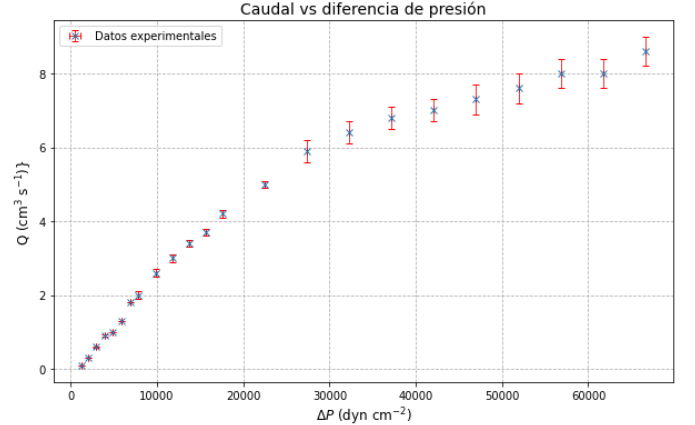
\includegraphics[width=\textwidth]{grafico_01x01_caudal_presion.png}
	\end{minipage}
	\begin{minipage}{0.46\textwidth} 
		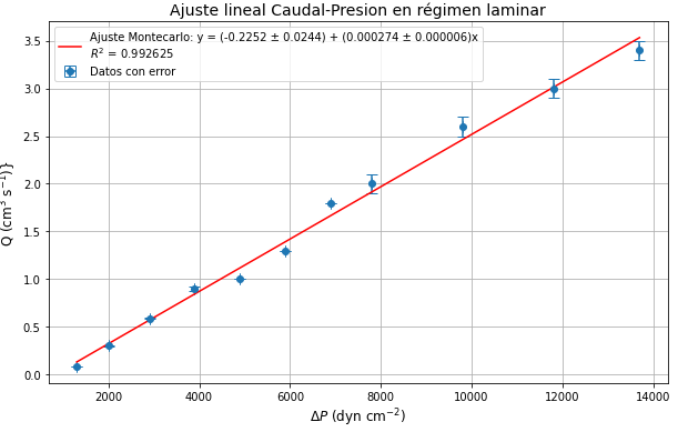
\includegraphics[width=\textwidth]{grafico_01x02_ajuste_lineal_caudal_presion.png}
	\end{minipage}
	\caption{ \footnotesize Gráfica de los datos de caudal y diferencia de presión calculados. {a) Totalidad de puntos b) Ajuste Linear solo en puntos con flujo laminar.}}
	\label{fig:qp}
\end{figure}
	
\begin{table}[h]		
	\centering
	\renewcommand{\arraystretch}{1.5} % Aumenta la altura de las celdas
	\begin{tabular}{|>{\centering\arraybackslash}m{1.5cm}|>{\centering\arraybackslash}m{2.5cm}|>{\centering\arraybackslash}m{5.5cm}|>{\centering\arraybackslash}m{5.5cm}|}
		\toprule
		\toprule
		\textbf{Variable} & \textbf{Función} & \textbf{Expresión de $\Delta$} & \textbf{Valor de $\Delta$} \\
		\hline
		$m_a$ & $m_a = m_T - m_v$ & $\Delta m_a = \left|\frac{\partial m_a}{\partial m_T}\right| \Delta m_T + \left|\frac{\partial m_a}{\partial m_v}\right| \Delta m_v$ & $\Delta m_a = 0.01 + 0.01 = 0.02$ \\
		\hline
		$V$ & $V = \frac{m_a}{\rho_a}$ & $\Delta V = \frac{\Delta m_a}{\rho_a}$ & $\Delta V = 0.02$ \\
		\hline
		$Q$ & $Q = \frac{V}{t}$ & $\Delta Q = \left|\frac{1}{t}\right| \Delta V + \left|\frac{-V}{t^2}\right| \Delta t$ & $\Delta Q = \frac{0.02}{10} + \frac{85.52}{10^2} \cdot 0.5 = 0.04$ \\
		\hline
		$h$ & $h = h_0 - h_m$ & $\Delta h = \left|\frac{\partial h}{\partial h_0}\right| \Delta h_0 + \left|\frac{\partial h}{\partial h_m}\right| \Delta h_m$ & $\Delta h = 0.1 + 0.1 = 0.2$ \\
		\hline
		$\Delta p$ & $\Delta p = \rho g h$ & $\Delta (\Delta p) = \rho g \Delta h$ & $\Delta (\Delta p) = 1 \times 980 \times 0.2 = 196 \approx 200$ \\
		\bottomrule
		\bottomrule
	\end{tabular}
	\caption{\footnotesize Tabla: Cálculos de propagación de errores para la tabla \ref{tab:medidas_1}}
	\label{tab:niceprop}
\end{table}


	
	
	\begin{figure}[H]
		\centering
		\begin{minipage}{0.42\textwidth} 
			\includegraphics[width=0.9\textwidth]{grafico_01x03_distribución regresion.png}
		\end{minipage}
		\caption{ \footnotesize Histograma de las pendientes de la regresiones simuladas para calculo de incertidumbres.}
		\label{fig:hist}
	\end{figure}

	
	Como se observa en la figura \ref{fig:qp}b, en régimen laminar el ajuste lineal es muy bueno, siendo la constante de proporcionalidad entre el caudal y la diferencia de presión ($Q=k\Delta P$) en los extremos del capilar de $k=(2.74\pm0.06$) cm$^5\cdot10^{-4}$ dyn$^{-1}$ s$^{-1}$. En la sección 1.5 se discuten e interpretan los resultados arrojados por estas gráficas.
	
	
	\vspace{\baselineskip} 
	
	De acuerdo a la expresión \ref{eq:velocidad_promedio}, para el cálculo de la velocidad es necesario el radio $R$ del capilar \ref{eq:radio}, el cual se determinará experimentalmente. Por tanto es necesario determinar la masa de agua $m_a$ contenida en el capilar lleno. Para ello se han realizado tres medidas de  la masa el tubo capilar lleno de agua, todo ello contenido en le vaso de llenado $m_{vca}$ que se ha empleado en la toma de datos anterior. Además se hicieron dos medidas el tubo capilar vacío $m_c$. En tabla \ref{tab:datos_r} se muestran estos datos y el valor promedio con su propagación de errores.
		
	\begin{equation}\label{eq:radio}
		V= L_c\pi R^2;\quad V=\frac{m_a}{\rho_a} \rightarrow R = \sqrt{\frac{m_a}{\rho\cdot \pi \cdot L_c}}
	\end{equation}
	
	
	La masa de agua es calculada como $m_a=m_{vca} - m_c - m_v$.
	
	\begin{table}[H]
		\centering
		\begin{minipage}{0.7\textwidth} 
			\centering
			\begin{tabular}{|c|c|c|c|c|}
				\toprule
				$m_{vca}$ (g) & 213.10$\pm$0.01  & 213.13$\pm$0.01 & 213.07$\pm$0.01 & \textbf{213.1$\pm$0.01}\\
				\hline
				$m_c$ (g) & 41.54$\pm$0.01 & 41.47$\pm$0.01 & - & \textbf{41.51$\pm$0.01} \\
				\hline
				$m_a$ (g) & 4.14$\pm$0.03 & 4.24$\pm$0.03 & - & \textbf{4.19$\pm$0.03} \\
				\bottomrule
			\end{tabular}
			\caption{\footnotesize Tabla con las medidas de masa necesarias para el calcula del capilar. Las incertidumbres son inmediatas.}
			\label{tab:datos_r}
		\end{minipage}
	\end{table}
	
	Por tanto sustituyendo en \ref{eq:radio}, obtenemos R=0.149. Para el calculo de su incertidumbre determinamos previamente $R^2$ que es el valor que aparece en la expresión de la velocidad. Esto facilita además el cálculo de la incertidumbre ya que $\Delta R^2 = \left|\frac{1}{\pi L_c}\right|\Delta m_a + \left|\frac{1}{\pi m_a L_c^2}\right|\Delta L_c = 0.000169$ cm. por tanto tenemos que  $R^2= (2.22\pm0.02)\cdot10^{-2}$ cm$^2$.
	
	\vspace{\baselineskip} 
	
	Dado que $R=\sqrt{R^2}\rightarrow \Delta R = \frac{\Delta R^2}{2R}$. Operando obtenemos $R = (1.49\pm0.03)\cdot10^{-1}$ cm.
	
	\vspace{\baselineskip} 
	Ahora estamos en disposición de calcular la viscosidad dinámica $\mu$ a partir de \ref{eq:hagen_poiseuille}\ref{eq:visco} ya que disponemos el valor de la pendiente $k$ del ajuste lineal para régimen laminar realizado anteriormente.
	

	\begin{equation}\label{eq:visco}
		\mu=\frac{\pi R^4}{8kL_c} \rightarrow \Delta \mu =  \frac{\pi}{8}\left(\left|\frac{2R^2}{8kL_c}\right|\Delta R^2 + \left|-\frac{R^4}{k^2L_c}\right|\Delta k + \left|-\frac{R^4}{kL_c^2}\right|\Delta L_c\right)
	\end{equation}
	
	Operando obtenemos $\mu= (1.19\pm0.03)\cdot10^{-2}$ dyn$\cdot$s$\cdot$ cm$^{-2}$ = (1.19\pm0.03) cP. Es importante señalar que aunque $\mu$ se calcula a partir de un régimen laminar, es una característica intrínseca de los fluidos.
	
    \vspace{\baselineskip} 
	Este dato nos permita ahora obtener las velocidades promedio $U$ y de ahí el número de reynolds $Re$ y  el coeficiente de rozamiento $\lambda$ para cada un $Q$ y $\Delta P$ dados (tabla \ref{tab:medidas_2}). En las expresiones \ref{eq:deltas}, se muestran las expresiones empleadas para la propagación de errores en estas variables. Esto nos permite crear el diagrama de Moody, figura \ref{fig:moody}, para los datos experimentales en comparación con los valores esperados para régimen laminar \ref{eq:laminar_friction} y turbulento \ref{eq:karman_prandtl}.
	
	
	
	\begin{equation}\label{eq:deltas}
		\begin{aligned}
			U &= \frac{Q}{\pi R^2} & \rightarrow \Delta U &= \left|\frac{1}{\pi R^2}\right| \Delta Q + \left|\frac{2Q}{\pi R^3}\right| \Delta R \\
			Re &= \frac{2 \rho U R}{\mu} & \rightarrow \Delta Re &= \frac{2UR}{\mu}\Delta \rho + \frac{2\rho R}{\mu}\Delta U + \frac{2\rho U}{\mu}\Delta R + \frac{2\rho UR}{\mu^2}\Delta \mu \\
			\lambda &= \frac{4 R \Delta p}{L \rho U^2} & \rightarrow \Delta \lambda &= \frac{4\Delta p}{L\rho U^2}\Delta R + \frac{4R}{L\rho U^2}\Delta(\Delta p) + \frac{4R\Delta p}{L^2\rho U^2}\Delta L  + \frac{8R\Delta p}{L\rho U^3}\Delta U
		\end{aligned}
	\end{equation}
	
	
	\begin{table}[H]
		\begin{minipage}{\textwidth}
			\centering
			\begin{tabular}{|C{1.8cm}|C{2cm}|C{2.5cm}|w{c}{2.5cm}|C{2.5cm}|}
				\toprule
				\toprule
				Q (cm$^3$s$^{-1}$) &
				$\Delta p = \rho g h$ { }(dyn$\cdot$cm$^{-2}$)  &
				$U = \frac{Q}{\pi R^2}$ (cm$\cdot$s$^{-1}$) &
				$Re = \frac{U\rho(2R)}{\mu}$& 
				$\lambda = \frac{4 R \Delta p}{L_c \rho U^2}$ \\
				\bottomrule
				\bottomrule
				$8.6 \pm 0.4$  & 66600$\pm$200 &    123$\pm$7  & 3090$\pm$255 &0.044 $\pm$ 0.005 \\\
				$8.0 \pm 0.4$  & 61700$\pm$200 &    114$\pm$7  & 2864$\pm$249 &0.047 $\pm$ 0.006 \\
				$8.0 \pm 0.4$  & 56800$\pm$200 &    114$\pm$7  & 2864$\pm$249 &0.043 $\pm$ 0.006 \\
				$7.6 \pm 0.4$  & 51900$\pm$200 &    109$\pm$7  & 2730$\pm$245 &0.043 $\pm$ 0.006 \\
				$7.3 \pm 0.4$  & 47000$\pm$200 &    104$\pm$7  & 2622$\pm$243 &0.043 $\pm$ 0.006 \\
				$7.0 \pm 0.3$  & 42100$\pm$200 &    100$\pm$5  & 2514$\pm$190 &0.042 $\pm$ 0.004 \\
				$6.8 \pm 0.3$  & 37200$\pm$200 &     97$\pm$5   & 2442$\pm$188&0.039 $\pm$ 0.004 \\
				$6.4 \pm 0.3$  & 32300$\pm$200 &  	 92$\pm$5  & 2298$\pm$184 & 0.038 $\pm$ 0.004 \\
				$5.9 \pm 0.3$  & 27400$\pm$200 &     84$\pm$5  & 2119$\pm$180 &0.039 $\pm$ 0.005 \\
				$5.0 \pm 0.1$  & 22500$\pm$200 &     72$\pm$2  & 1796$\pm$96  &0.043 $\pm$ 0.003 \\
				$4.2 \pm 0.1$  & 17600$\pm$200 &     60$\pm$2  & 1508$\pm$89  &0.049 $\pm$ 0.004 \\
				$3.7 \pm 0.1$  & 15700$\pm$200 &     53$\pm$2  & 1329$\pm$84  &0.056 $\pm$ 0.005 \\
				$3.4 \pm 0.1$  & 13700$\pm$200 &     49$\pm$2  & 1221$\pm$81  &0.057 $\pm$ 0.006 \\
				$3.0 \pm 0.1$  & 11800$\pm$200 &     43$\pm$2  & 1077$\pm$78  &0.063 $\pm$ 0.007 \\
				$2.6 \pm 0.1$  &  9800$\pm$200 &     37$\pm$2  &  934$\pm$74  &0.071 $\pm$ 0.009 \\
				$2.0 \pm 0.1$  &  7800$\pm$200 &     29$\pm$2  &  718$\pm$69  &0.092 $\pm$ 0.015 \\
				$1.8 \pm 0.0$  &  6900$\pm$200 &   25.7$\pm$0.2 &  646$\pm$21 &0.104 $\pm$ 0.005 \\
				$1.3 \pm 0.0$  &  5900$\pm$200 &   18.6$\pm$0.1 &  467$\pm$14 &0.17 $\pm$ 0.008 \\
				$1.0 \pm 0.0$  &  4900$\pm$200 &   14.3$\pm$0.1 &  359$\pm$12 &0.238 $\pm$ 0.013 \\
				$0.90\pm 0.02$ &  3900$\pm$200 &   12.9$\pm$0.4 &  324$\pm$18 &0.233 $\pm$ 0.027 \\
				$0.59\pm 0.01$ &  2900$\pm$200 &    8.4$\pm$0.2 &  211$\pm$10 &0.409 $\pm$ 0.048 \\
				$0.30\pm 0.01$ &  2000$\pm$200 &    4.3$\pm$0.2 &  108$\pm$8  &1.076 $\pm$ 0.21 \\
				$0.08\pm 0.00$ &  1300$\pm$200 &   1.14$\pm$0.00&   29$\pm$1  &9.953 $\pm$ 1.548 \\
				\bottomrule
				\bottomrule		
			\end{tabular}
			\caption{ \footnotesize Medidas y cálculos previos derivados de la determinación del régimen de velocidades del agua en el tubo capilar.}
			\label{tab:medidas_2}
		\end{minipage}
	\end{table}

	\begin{figure}[H]
		\centering
		\begin{minipage}{0.75\textwidth} 
			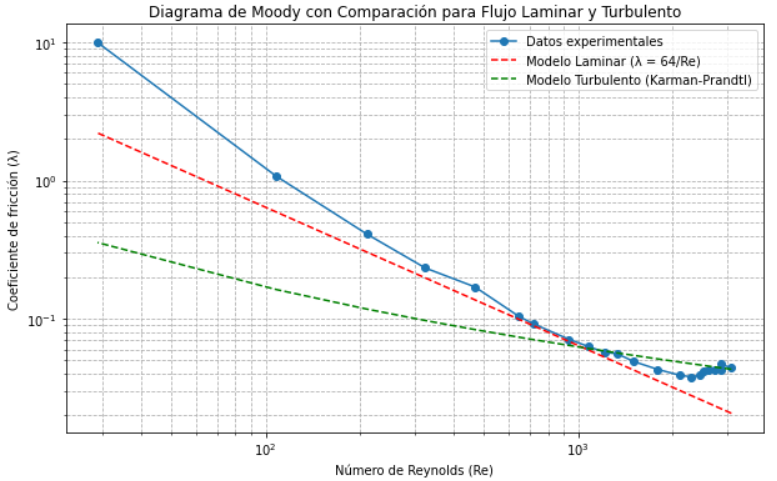
\includegraphics[width=0.9\textwidth]{grafico_01x04_diagrama_moody.png}
		\end{minipage}
		\caption{ \footnotesize Diagramas de Moody para los datos experimentales en contraste con los curvas en régimen laminar y en régimen turbulento.}
		\label{fig:moody}
	\end{figure}

	\section{Discusión}
	
	En  la figura \ref{fig:qp}a, donde se enfrenta el caudal y la diferencia de presión en los extremos del tubo capilar, se ilustran dos regímenes de flujo distintos: el flujo laminar y la transición hacia la turbulencia. Inicialmente, se observa un comportamiento lineal entre el caudal (\( Q \)) y la diferencia de presión (\( \Delta P \)), característico del régimen laminar, donde la ley de Hagen-Poiseuille es aplicable. En este régimen, el flujo es ordenado y las partículas del fluido se mueven en capas paralelas. Sin embargo, a medida que la diferencia de presión aumenta, la gráfica comienza a desviarse de la linealidad, indicando que el flujo está entrando en un régimen transitorio. Este cambio sugiere la aparición de inestabilidades que eventualmente conducen al flujo turbulento, donde las fuerzas inerciales superan a las viscosas y el patrón de flujo se vuelve caótico. La segunda gráfica, figura \ref{fig:qp}b, que considera solos los dato donde se observa régimen laminar, confirma la linealidad de esta fase, excluyendo los datos que corresponden a la transición hacia la turbulencia. El excelente ajuste lineal, con un coeficiente de determinación ($R^2=0.9926$), confirma la validez de la ley de Hagen-Poiseuille en este régimen.
	
	\vspace{\baselineskip}
	
	La medición de la viscosidad dinámica del agua a 19.4°C arrojó un resultado de $1.19\pm0.03$ cP, aproximadamente un 19\% mayor que el valor bibliográfico  de 1.002 cP. Esta discrepancia, aunque significativa, no invalida el método experimental basado en la medición del caudal y la diferencia de presión en un tubo capilar. La sensibilidad en cálculo de la pendiente  $k$ en la regresión lineal, figura \ref{fig:qp} pone de manifiesto lo relevante de una selección de los puntos pertenecientes al  régimen laminar. Esto sin menoscabar la importancia de considerar factores como la pureza del agua, el control preciso de la temperatura y los posibles efectos no lineales en el flujo capilar. 
	
	\vspace{\baselineskip}
	
	En el diagrama de Moody, figura \ref{fig:moody}, los datos experimentales muestran una concordancia aceptable con los modelos de flujo laminar y turbulento, aunque con matices. En el rango de números de Reynolds bajos (600-1500), se observa un buen ajuste  de los datos al modelo laminar, corroborando la validez de la ecuación λ = 64/Re en este régimen. La desviación posterior de los datos experimentales de este modelo, ocurre aproximadamente en Re ≈ 2000-3000, que indica la región de transición hacia el flujo turbulento. Esta transición, caracterizada por su naturaleza gradual, es consistente con las observaciones típicas en la mecánica de fluidos experimental. A medida que el número de Reynolds aumenta más allá de 3000, los datos convergen hacia el modelo turbulento de Kármán-Prandtl, aunque se evidencian discrepancias menores. Estas variaciones pueden atribuirse a factores intrínsecos al experimento, como la rugosidad superficial del conducto o fluctuaciones en las condiciones del flujo. La dispersión observada en los datos, particularmente en la zona de transición y en el régimen turbulento, es congruente con las incertidumbres inherentes a este tipo de mediciones experimentales.
	
	
	\vspace{\baselineskip} 


	\section{Conclusiones}
	
	 Los datos experimentales tomados han permitido verificar dos aspectos clave del comportamiento de fluidos en conductos. Primero, se ha confirmado la validez de la ley de Hagen-Poiseuille en el régimen laminar, evidenciada por la relación lineal entre el caudal y la diferencia de presión. Segundo, se ha identificado claramente la transición del flujo laminar al flujo turbulento a medida que la presión aumenta, lo que refleja el cambio en el comportamiento del fluido, tal como predice la teoría de la dinámica de fluidos. Por tanto  el  experimento ha logrado caracterizar adecuadamente los regímenes de flujo en función de la diferencia de presión aplicada.
	 
	 \vspace{\baselineskip}
	 
	 El experimento de medición de la viscosidad dinámica del agua mediante flujo capilar revela tanto las posibilidades como las limitaciones de las mediciones precisas en física de fluidos. El método es aplicable, pero la variabilidad en los resultados indica la necesidad de un diseño experimental cuidadoso y un análisis estadístico detallado.
	
	 \vspace{\baselineskip}
	 
	 Mediante el diagrama de Moody se han contrastado con los datos experimentales de fricción en el capilar con los que cabría esperar en los regímenes laminar y turbulento, mostrando un ajuste parcial para ciertos rangos de número de Reynolds.
	 
	 \vspace{\baselineskip}  
	
	 Finalmente, el experimento llevado avala el marco teórico clásico de la física de fluidos en conductos.
	 
	
	\begin{thebibliography}{99}
	
	\bibitem{Jones1924}
	 White, F. M. (2004). Mecánica de Fluidos (5ª ed.). McGraw-Hill.
	
	
	\bibitem{villasante}
	 Losada Villasante, A. (2010). Hidráulica de Riegos (2ª ed.). Mundi-Prensa..
	
	\bibitem{Anderson_montecarlo} Anderson, G. M., \textit{Error propagation by the Monte Carlo method in geochemical calculations}, Geochimica et Cosmochimica Acta, 40(12), 1533-1538, 1976

	\bibitem{error_prop} Bevington, Philip R., y D. Keith Robinson. \textit{Data Reduction and Error Analysis for the Physical Sciences}. 3ra ed., McGraw-Hill, 2003.
	
	
\end{thebibliography}


\clearpage
		

	
% Segundo artículo
\titleformat{\chapter}[display]
{\normalfont\bfseries}{}{0pt}{\LARGE}
\chapter{Relación de dispersión de ondas de tensión superficial.}
\begin{abstract}
	\vspace{0.5cm}
	\footnotesize{En este trabajo se ha llevado a cabo una estimación  de la tensión superficial del agua mediante difracción láser por ondas capilares. Se observó una fuerte relación lineal entre la frecuencia angular al cuadrado y el número de onda al cubo, validando la teoría subyacente. Aunque los resultados mostraron consistencia interna, el valor obtenido difiere significativamente del de referencia. Se discuten las posibles fuentes de error y se proponen mejoras para futuros experimentos. El estudio demuestra el potencial del método, destacando áreas para refinar su precisión.}
	
\end{abstract}
\section{Introducción}
% ***************************************

El estudio de la tensión superficial y las ondas capilares tiene sus raíces en las observaciones científicas del siglo XVII, aunque el concepto no se comprendía completamente en ese entonces.

\vspace{\baselineskip}

En 1805, Thomas Young dio un paso significativo al introducir formalmente el concepto de tensión superficial en su ensayo 'An Essay on the Cohesion of Fluids'. Young describió la tensión superficial como una fuerza que actúa en la superficie de un líquido, perpendicular a cualquier línea trazada en la superficie.

\vspace{\baselineskip}

Un año después, Pierre-Simon Laplace complementó el trabajo de Young desarrollando la teoría matemática de la capilaridad en su obra "Mécanique Céleste". Laplace explicó cómo la tensión superficial causa que los líquidos suban por tubos capilares. La combinación de los trabajos de Young y Laplace llevó a la formulación de la ecuación de Young-Laplace, que se convirtió en un pilar fundamental en el estudio de la tensión superficial.

\vspace{\baselineskip}

En 1830, el físico alemán Franz Ernst Neumann contribuyó significativamente al campo al derivar la ecuación que relaciona la tensión superficial con la energía libre de superficie. Este trabajo estableció una base termodinámica sólida para el concepto de tensión superficial.

\vspace{\baselineskip}

El estudio de las ondas capilares, estrechamente relacionado con la tensión superficial, avanzó considerablemente en la segunda mitad del siglo XIX. William Thomson (Lord Kelvin) en 1871 y Joseph Boussinesq en 1913 derivaron independientemente la relación de dispersión para ondas capilares. Esta relación, crucial para nuestro experimento, describe cómo la frecuencia de las ondas capilares depende de su longitud de onda y de las propiedades del fluido.

\vspace{\baselineskip}

El siglo XX trajo consigo avances tecnológicos que permitieron estudios más detallados de la tensión superficial y las ondas capilares. En la década de 1960, la introducción de la luz láser en el estudio de fenómenos de superficie revolucionó el campo, permitiendo mediciones más precisas de la tensión superficial y las propiedades de las ondas capilares.

\vspace{\baselineskip}

El método experimental que utilizamos en esta práctica, basado en la difracción de luz láser por ondas capilares, se desarrolló y refinó en las últimas décadas del siglo XX. Este método combina principios de óptica física con la teoría de ondas capilares, permitiendo mediciones precisas de la tensión superficial sin necesidad de contacto directo con la superficie del líquido.

\vspace{\baselineskip}

En la actualidad, el estudio de la tensión superficial y las ondas capilares sigue siendo un campo activo de investigación, con aplicaciones en diversas áreas como la física de fluidos, la química de superficies, la biología molecular y la tecnología de microfluidos.


\section{Fundamento teórico}
% ***************************************


La superficie de un fluido está sometida a dos fuerzas principales: la tensión superficial y la gravedad. Cuando se produce una perturbación en la superficie, estas fuerzas actúan como fuerzas recuperadoras, generando dos tipos de ondas: ondas de gravedad y ondas capilares.

\vspace{\baselineskip}

Las ondas de gravedad se deben a la presencia del campo gravitatorio. Una vez que la superficie libre de un fluido en reposo ha sido perturbada, la diferencia de altura entre distintos puntos de la superficie del fluido da origen a diferencias de presión hidrostática consecuencia de la gravedad.

\vspace{\baselineskip}

Por otro lado, las ondas capilares son consecuencia de las fuerzas de tensión superficial que experimentan las moléculas de la superficie del fluido. La magnitud de la fuerza de tensión superficial por unidad de superficie es $\sigma k$, donde $\sigma$ es la tensión superficial y $k$ es el número de onda.

\vspace{\baselineskip}


En la práctica, las ondas en la superficie de un fluido son una combinación de estos dos efectos. La importancia relativa de cada uno depende de la longitud de onda de la perturbación. Para ondas de longitud de onda larga, los efectos de la gravedad dominan, mientras que para ondas de longitud de onda corta, los efectos de la tensión superficial son más importantes.

\vspace{\baselineskip}

A partir de las ecuaciones de Navier-Stokes y aplicando las condiciones de contorno de Young-Laplace se llaga a una relación de dispersión que  describe cómo la frecuencia angular $\omega$ de las ondas depende del número de onda $k$. Para ondas en la superficie libre de un fluido, considerando tanto los efectos de la gravedad como los de la tensión superficial, la relación de dispersión general tiene la forma:

\begin{equation}
	\omega^2 = (gk + \frac{\sigma}{\rho}k^3)\tanh(kh)
	\label{eq:dispersion_general}
\end{equation}

donde $h$ es la profundidad del fluido. 

\vspace{\baselineskip}

En nuestro experimento, trabajamos con una profundidad de agua suficiente para considerarla como ''aguas profundas'' en relación con las longitudes de onda que estamos generando. En este caso, $\tanh(kh) \approx 1$, y la ecuación se simplifica a:

\begin{equation}
	\omega^2 = gk + \frac{\sigma}{\rho}k^3
	\label{eq:dispersion_simplificada}
\end{equation}

Además, nos enfocamos en ondas de longitud de onda muy corta, donde los efectos de la tensión superficial dominan sobre los efectos de la gravedad. En este régimen, podemos despreciar el término $gk$, lo que nos lleva a la relación de dispersión para ondas de tensión superficial puras:

\begin{equation}
	\omega^2(k) = \frac{\sigma}{\rho} k^3
	\label{eq:dispersion}
\end{equation}

Esta es la ecuación que utilizaremos en nuestro análisis experimental para determinar la tensión superficial del agua.


\vspace{\baselineskip}

Para determinar experimentalmente la relación de dispersión, se generan ondas estacionarias en la superficie del líquido mediante un transmisor mecánico acoplado a un generador de señales. Se ilumina la superficie con un haz de luz láser monocromática, y el patrón de difracción resultante se observa en una pantalla.

\vspace{\baselineskip}

El patrón de difracción consiste en un máximo central y varios máximos secundarios. La posición angular de estos máximos permite calcular el número de onda $k$ mediante la siguiente ecuación:

\vspace{\baselineskip}

\begin{equation}
	k_n = \frac{\pi}{n \lambda}(\theta_n - \theta_{-n}) \theta_0
	\label{eq:numero_onda}
\end{equation}

\vspace{\baselineskip}

donde $n$ es el orden del máximo secundario, $\lambda$ es la longitud de onda del láser, $\theta_n$ y $\theta_{-n}$ son los ángulos de los máximos secundarios de orden $n$, y $\theta_0$ es el ángulo del máximo central.

\vspace{\baselineskip}

En la práctica, se utiliza la aproximación paraxial para ángulos pequeños, lo que permite expresar los ángulos en términos de distancias medidas en el montaje experimental:

\vspace{\baselineskip}

\begin{equation}
	\theta_0 \approx \frac{b}{a}
	\label{eq:theta0}
\end{equation}

\begin{equation}
	\theta_n - \theta_{-n} \approx \frac{c_n}{a}
	\label{eq:thetan}
\end{equation}

\vspace{\baselineskip}

donde $a$ es la distancia horizontal del punto de incidencia del láser a la pantalla, $b$ es la distancia vertical del máximo central a la proyección del punto de incidencia, y $c_n$ es la distancia entre los máximos secundarios de orden $n$.

\vspace{\baselineskip}

La frecuencia angular $\omega$ se relaciona con la frecuencia $f$ del generador de señales mediante:

\begin{equation}
	\omega = 2\pi f
	\label{eq:omega}
\end{equation}

\vspace{\baselineskip}

Al medir $k$ y $\omega$ para diferentes frecuencias, se puede representar gráficamente $\omega^2$ vs $k^3$. Según la relación de dispersión (ecuación \ref{eq:dispersion}), esta gráfica debe ser una línea recta cuya pendiente es $\frac{\sigma}{\rho}$. Conociendo la densidad del líquido, se puede determinar la tensión superficial $\sigma$.

\vspace{\baselineskip}

Para determinar el rango de validez de nuestro experimento, comparamos la fuerza por unidad de volumen de las ondas capilares ($\sigma k^2$) con la de las ondas de gravedad ($\rho g$). Los efectos de la gravedad se pueden despreciar cuando:

\vspace{\baselineskip}

\begin{equation}
	\sigma k^2 \gg \rho g
	\label{eq:validez}
\end{equation}

\vspace{\baselineskip}

Esta comparación nos permite establecer el límite inferior del número de onda para el cual nuestro análisis de ondas capilares es válido, utilizando las ecuaciones \ref{eq:numero_onda}, \ref{eq:theta0} y \ref{eq:thetan} para calcular $k$ experimentalmente.


\section{Metodología}

\subsection{Descripción del experimento}

\begin{enumerate}
	\item Se coloca un recipiente lleno hasta el borde con agua destilada. El recipiente debe quedar horizontal y en una superficie con el menor número de vibraciones posibles. Se toma nota  la temperatura del agua la cual se obtiene de forma indirecta  a partir de la temperatura ambiente del laboratorio al permanecido ésta suficiente tiempo  contacto con el aire como para alcanzar equilibrio térmico con el aire. ($T_a=24\pm1$)
	\item Se coloca el segmento horizontal del transmisor de tal forma que contacte paralelamente con la superficie del agua
	\item Se hace incidir un haz de luz láser ($\lambda=663$ nm) sobre la superficie del agua de tal forma que su reflejo se observe en una pantalla colocada previamente a una distancia grande del recipiente. El punto de incidencia en el agua debe rebasar ligeramente el segmento horizontal del transmisor mecánico, figura \ref{fig:esquema}.
	\item Se conecta el generador de señales a una frecuencia de 150 Hz
	\item Se ajusta la amplitud de la onda estacionaria hasta observar el patrón de difracción en la pantalla,figura \ref{fig:estdif}.
	\item Con ayuda de un papel milimétrico, se calcula la distancia entre máximos de primer, segundo y tercer orden (si se observan). Se recomienda tomar una fotografía. 
	\item Se repiten los pasos 5 y 6 variando la frecuencia del generador de 150 a 400 Hz en pasos de 10 Hz y anotando el valor de la distancia entre máximos para cada frecuencia.
	\item Se miden las distancias horizontal y vertical del punto de incidencia a la pantalla. Se emplea distanciómetro láser ($\Delta = \pm0.001$ m) y un cinta métrica ($\Delta=\pm0.001$ m)
\end{enumerate}


\begin{figure}[H]
	\centering
	\begin{minipage}{0.95\textwidth} 
		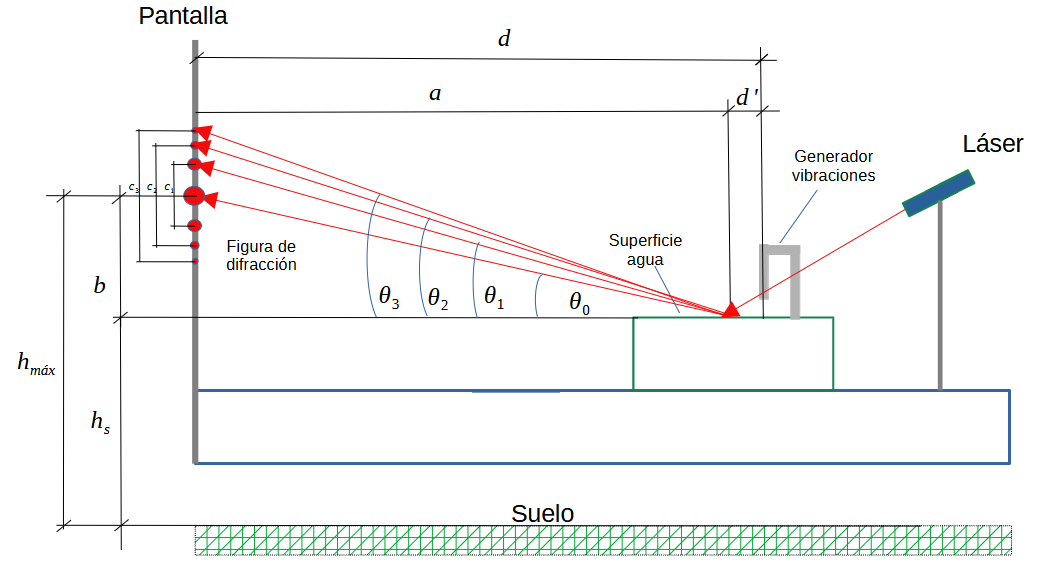
\includegraphics[width=0.9\textwidth]{grafico_02x01_esquema_montaje.png}
	\end{minipage}
	\caption{ \footnotesize Esquema del montaje con los parámetros geométricos involucrados.}
	\label{fig:esquema}
\end{figure}



\begin{figure}[H]
	\centering
	\begin{minipage}{0.40\textwidth} 
		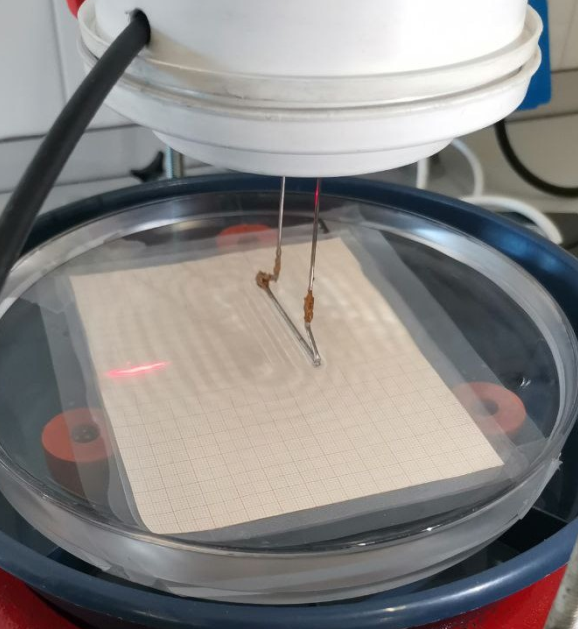
\includegraphics[width=\textwidth]{grafico_02x02_ondas_stacionarias.png}
		\centering(a)
	\end{minipage}
	\hspace{0.5cm}
	\begin{minipage}{0.45\textwidth} 
		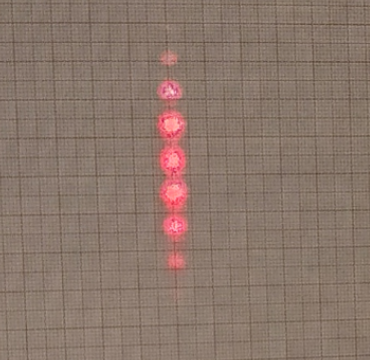
\includegraphics[width=1\textwidth]{grafico_02x03_figura_difraccion.png}
		\centering (b)
	\end{minipage}
	\caption{ \footnotesize {a) Ondas estacionarias en la superficie del agua b) Figura de difracción generada.}}
	\label{fig:estdif}
\end{figure}

\subsection{Propagación de errores}

En lo que se refiere a la propagación de errores, los valores de error absoluto se han obtenido por la expresión general de propagación lineal de errores para una función $f=f(x_1,x_2...x_n)$, donde cada variable $x_i$  es independiente y las incertidumbres en las medidas son $\Delta x_1, \Delta x_2,....\Delta x_n$. En estas condiciones el valor de $\Delta f$ viene dado por la ecuación ~\ref{eq:properr_1}. 


\begin{equation}\label{eq:properr_1}
	{\Delta f} = \left|\mathbf{\nabla}f\right|\cdot\mathbf{\Delta x} =  \sum_{i=1}^{n}\left|\frac{\partial f}{\partial x_i}\right|\Delta x_i
\end{equation}


\vspace{\baselineskip}
Para los ajustes por regresión lineal se utilizó el método de Montecarlo \cite{Anderson_montecarlo}, generando datos aleatorios (distribución normal) dentro del rango de la incertidumbre de los datos, tomando como valor central el valor de la  variable. Se realizaron 10,000 simulaciones, tomando como valor medio de los parámetros el promedio de todas las simulaciones y como incertidumbre, la desviación típica.

\section{Resultados}

En primer lugar, de acuerdo al esquema \ref{fig:esquema}, necesitamos determinar los parámetros $a$ y $b$ para obtener $\theta$. En la tabla \ref{tab:medidas_ab}, se muestran las  medidas realizadas para su estimación. La estimación final se ha realizado promediando valores e incertidumbres de respectivas series de medidas.


\begin{table}[H]
	\centering
	\begin{minipage}{1\textwidth} 
		\centering
		\begin{tabular}{|c|c|c||c|c|c|}
			\toprule
			d (m) & d'(m) & a = d-d' (m) & $h_{max}$ (m) & $h_s$ (m) & b = $h_{max}-h_s$  (m) \\
			\hline
			3.854$\pm$0.001(*) &       -         & 3.854$\pm$0.001 (*) &  & & \\
			\hline
			3.874$\pm$0.001 & 0.020$\pm$0.001 & 3.854$\pm$0.002 &  & & \\
			\hline
			3.874$\pm$0.001 & 0.023$\pm$0.001 & 3.851$\pm$0.002 & 1.584$\pm$0.001 & 1.060$\pm$0.001 & 0.524$\pm$0.002\\
			\hline
			3.874$\pm$0.001 & 0.027$\pm$0.001 & 3.847$\pm$0.002 &1.580$\pm$0.001 & 1.065$\pm$0.001 & 0.515$\pm$0.002\\
			\hline
			3.874$\pm$0.001 & 0.026$\pm$0.001 & 3.858$\pm$0.002 &1.560$\pm$0.001 & 1.054$\pm$0.001 & 0.506$\pm$0.002\\
			\hline
			& & \textbf{3.851$\pm$0.002} & & & \textbf{0.515$\pm$0.002}\\
			\bottomrule
		\end{tabular}
		\caption{\footnotesize a) Serie de medidas realizadas para estimar el la distancia $a$ y $b$  y valor final estimado con su incertidumbre (en negrita). (*) Dato tomado con distanciómetro láser desde el punto de reflexión.}
		\label{tab:medidas_ab}
	\end{minipage}
\end{table}

\begin{table}[H]
	\centering
	\begin{minipage}{\textwidth} 
		\begin{tabular}{C{1.5cm}|C{2cm}| C{1.8cm}|C{2cm}| C{1.8cm}|C{2cm}|C{1.8cm}}
			\toprule
			\toprule
			$f$  (Hz) &
			$c_1$  (m) & 
			$k_1$ (m$^{-1}$)& 
			$c_2$ (m)&
			$k_2$ (m$^{-1}$)&
			$c_3$ (m)&
			$k_3$ (m$^{-1}$) \\
			\bottomrule
			\bottomrule
			150 $\pm$1 &	0.015$\pm$0.001 & 2500$\pm$ 200 & 0.028$\pm$0.001 &2300$\pm$ 100 & -               & -              \\
			160	$\pm$1 &	0.015$\pm$0.001 & 2500$\pm$ 200 & 0.029$\pm$0.001 &2400$\pm$ 100 & -               & -              \\
			170	$\pm$1 &	0.015$\pm$0.001 & 2500$\pm$ 200 & 0.030$\pm$0.001 &2500$\pm$ 100 & -               & -              \\
			180	$\pm$1 &	0.016$\pm$0.001 & 2600$\pm$ 200 & 0.031$\pm$0.001 &2600$\pm$ 100 & 0.046$\pm$0.001 & 2500$\pm$100   \\
			190	$\pm$1 &	0.016$\pm$0.001 & 2600$\pm$ 200 & 0.032$\pm$0.001 &2600$\pm$ 100 & 0.048$\pm$0.001 & 2600$\pm$100   \\
			200	$\pm$1 &	0.017$\pm$0.001 & 2800$\pm$ 200 & 0.034$\pm$0.001 &2800$\pm$ 100 & 0.050$\pm$0.001 & 2800$\pm$100   \\
			210	$\pm$1 &	0.018$\pm$0.001 & 3000$\pm$ 200 & 0.035$\pm$0.001 &2900$\pm$ 100 & 0.052$\pm$0.001 & 2900$\pm$100   \\
			220	$\pm$1 &	0.018$\pm$0.001 & 3000$\pm$ 200 & 0.036$\pm$0.001 &3000$\pm$ 100 & 0.055$\pm$0.001 & 3000$\pm$100   \\
			230	$\pm$1 &	0.019$\pm$0.001 & 3100$\pm$ 200 & 0.039$\pm$0.001 &3200$\pm$ 100 & 0.062$\pm$0.001 & 3400$\pm$100  \\
			240	$\pm$1 &	0.019$\pm$0.001 & 3100$\pm$ 200 & 0.038$\pm$0.001 &3100$\pm$ 100 & 0.053$\pm$0.001 & 2900$\pm$100   \\
			250	$\pm$1 &	0.020$\pm$0.001 & 3300$\pm$ 200 & 0.039$\pm$0.001 &3200$\pm$ 100 & 0.058$\pm$0.001 & 3200$\pm$100   \\
			260	$\pm$1 &	0.020$\pm$0.001 & 3300$\pm$ 200 & 0.040$\pm$0.001 &3300$\pm$ 100 & 0.061$\pm$0.001 & 3400$\pm$100  \\
			270	$\pm$1 &	0.021$\pm$0.001 & 3500$\pm$ 200 & 0.042$\pm$0.001 &3500$\pm$ 100 & 0.063$\pm$0.001 & 3500$\pm$100  \\
			280	$\pm$1 &	0.021$\pm$0.001 & 3500$\pm$ 200 & 0.042$\pm$0.001 &3500$\pm$ 100 & 0.062$\pm$0.001 & 3400$\pm$100  \\
			290	$\pm$1 &	0.022$\pm$0.001 & 3600$\pm$ 200 & 0.044$\pm$0.001 &3600$\pm$ 100 & 0.063$\pm$0.001 & 3500$\pm$100  \\
			300	$\pm$1 &	0.023$\pm$0.001 & 3800$\pm$ 200 & 0.046$\pm$0.001 &3800$\pm$ 100 & 0.067$\pm$0.001 & 3700$\pm$100  \\
			310	$\pm$1 &	0.023$\pm$0.001 & 3800$\pm$ 200 & 0.046$\pm$0.001 &3800$\pm$ 100 & 0.068$\pm$0.001 & 3700$\pm$100  \\
			320	$\pm$1 &	0.023$\pm$0.001 & 3800$\pm$ 200 & 0.047$\pm$0.001 &3900$\pm$ 100 & 0.069$\pm$0.001 & 3800$\pm$100  \\
			330	$\pm$1 &	0.024$\pm$0.001 & 4000$\pm$ 200 & 0.048$\pm$0.001 &4000$\pm$ 100 & 0.071$\pm$0.001 & 3900$\pm$100  \\
			340	$\pm$1 &	0.024$\pm$0.001 & 4000$\pm$ 200 & 0.049$\pm$0.001 &4000$\pm$ 100 & 0.074$\pm$0.001 & 4100$\pm$100  \\
			350	$\pm$1 &	0.025$\pm$0.001 & 4100$\pm$ 200 & 0.049$\pm$0.001 &4000$\pm$ 100 & 0.073$\pm$0.001 & 4000$\pm$100  \\
			360	$\pm$1 &	0.026$\pm$0.001 & 4300$\pm$ 200 & 0.050$\pm$0.001 &4100$\pm$ 100 & -               & -          \\
			370	$\pm$1 &	0.025$\pm$0.001 & 4100$\pm$ 200 & 0.051$\pm$0.001 &4200$\pm$ 100 & 0.077$\pm$0.001 & 4200$\pm$100  \\
			380	$\pm$1 &	0.026$\pm$0.001 & 4300$\pm$ 200 & 0.052$\pm$0.001 &4300$\pm$ 100 & 0.079$\pm$0.001 & 4400$\pm$100  \\
			390	$\pm$1 &	0.027$\pm$0.001 & 4500$\pm$ 200 & 0.054$\pm$0.001 &4500$\pm$ 100 & 0.08$\pm$0.001  & 4400$\pm$100  \\
			400	$\pm$1 &	0.026$\pm$0.001 & 4300$\pm$ 200 & 0.054$\pm$0.001 &4500$\pm$ 100 & 0.081$\pm$0.001 & 4500$\pm$100  \\
			\bottomrule
			\bottomrule		
		\end{tabular}
		\caption{ \small Datos tomados experimentalmente de las distancias $c_n$  entren máximos del mismo orden de magnitud para distintas frecuencias. Valores calculados del número de ondas $_n$ asociado a cada orden de difracción.}
		\label{tab:cks}
	\end{minipage}
\end{table}

\clearpage

Por tanto podemos calcular $\theta$ en la aproximación paraxial, de acuerdo a \ref{eq:theta}.

\vspace{\baselineskip}
\begin{equation}\label{eq:theta}
	\theta = \frac{b}{a} \rightarrow \Delta \theta = \frac{b}{a^2}\Delta a + \frac{\Delta b}{a}; \quad \theta = 0.1337\pm0.0006 \text{ rad}
\end{equation}


\vspace{\baselineskip}






Finalmente solo queda aplicar la ecuación \ref{eq:dispersion}. Por tanto es necesario calcular $\omega^2$ y las $k_n^4$ y sus respectivas incertidumbres y así llevar a cabo posteriormente un ajuste por regresión lineal. Las incertidumbres respectivas son las indicadas en \ref{eq:ldeltas2}.

\vspace{\baselineskip}

\begin{equation}\label{eq:ldeltas2}
	(\omega)^2 = (2\pi f)^2;\quad \Delta\omega^2=8\pi^2 f\Delta f;\quad  k_n^3 \rightarrow \Delta k_n^3= 3k^2\Delta k_n
\end{equation}

\vspace{\baselineskip}

La pendiente de la recta de ajuste nos dará la estimación de la tensión superficial del agua $\sigma$. Dado que hemos tomado medidas de hasta máximos de orden tres en el patrón de difracción tendremos tres estimaciones diferentes. 

\vspace{\baselineskip}
\begin{table}[H]
	
	\begin{minipage}{\textwidth} 
		\centering
		\begin{tabular}{C{1.5cm}|C{3.4cm}| C{2.2cm}|C{2.2cm}| C{2.2cm}}
	
			\toprule
			\toprule
			$f$  (Hz) &
			$\omega^2 = 4\pi^2f^2$ (rad$^2$s$^{-2}$) & 
			$k_1^3$ (m$^{-3}$)& 
			$k_2^3$ (m$^{-3}$) &
			$k_3^3$ (m$^{-3}$) \\
			\bottomrule
			\bottomrule
			150 $\pm$1 &	 (8.9$\pm$0.1$\cdot 10^5$) &(1.6$\pm$0.4$\cdot 10^{10}$) &(1.2$\pm$0.2$\cdot 10^{10}$) & -  \\
			160	$\pm$1 &	(10.1$\pm$0.1$\cdot 10^5$  &(1.6$\pm$0.4$\cdot 10^{10}$) &(1.4$\pm$0.2$\cdot 10^{10}$) & - \\
			170	$\pm$1 &	(11.4$\pm$0.1$\cdot 10^5$  &(1.6$\pm$0.4$\cdot 10^{10}$) &(1.6$\pm$0.2$\cdot 10^{10}$) & -  \\
			180	$\pm$1 &	(12.8$\pm$0.1)$\cdot 10^5$ &(1.8$\pm$0.4$\cdot 10^{10}$) &(1.8$\pm$0.2$\cdot 10^{10}$) &(1.6$\pm$0.2$\cdot 10^{10}$)   \\
			190	$\pm$1 &	(14.3$\pm$0.2)$\cdot 10^5$ &(1.8$\pm$0.4$\cdot 10^{10}$) &(1.8$\pm$0.2$\cdot 10^{10}$) &(1.8$\pm$0.2$\cdot 10^{10}$)   \\
			200	$\pm$1 &	(15.8$\pm$0.2)$\cdot 10^5$ &(2.2$\pm$0.5$\cdot 10^{10}$) &(2.2$\pm$0.2$\cdot 10^{10}$) &(2.2$\pm$0.2$\cdot 10^{10}$)   \\
			210	$\pm$1 &	(17.4$\pm$0.2)$\cdot 10^5$ &(2.7$\pm$0.5$\cdot 10^{10}$) &(2.4$\pm$0.3$\cdot 10^{10}$) &(2.4$\pm$0.3$\cdot 10^{10}$)   \\
			220	$\pm$1 &	(19.1$\pm$0.2)$\cdot 10^5$ &(2.7$\pm$0.5$\cdot 10^{10}$) &(2.7$\pm$0.3$\cdot 10^{10}$) &(2.7$\pm$0.3$\cdot 10^{10}$)   \\
			230	$\pm$1 &	(20.9$\pm$0.2)$\cdot 10^5$ &(3.0$\pm$0.6$\cdot 10^{10}$) &(3.3$\pm$0.3$\cdot 10^{10}$) &(3.9$\pm$0.3$\cdot 10^{10}$)  \\
			240	$\pm$1 &	(22.7$\pm$0.2)$\cdot 10^5$ &(3.0$\pm$0.6$\cdot 10^{10}$) &(3.0$\pm$0.3$\cdot 10^{10}$) &(2.4$\pm$0.3$\cdot 10^{10}$)   \\
			250	$\pm$1 &	(24.7$\pm$0.2)$\cdot 10^5$ &(3.6$\pm$0.7$\cdot 10^{10}$) &(3.3$\pm$0.3$\cdot 10^{10}$) &(3.3$\pm$0.3$\cdot 10^{10}$)   \\
			260	$\pm$1 &	(26.7$\pm$0.2)$\cdot 10^5$ &(3.6$\pm$0.7$\cdot 10^{10}$) &(3.6$\pm$0.3$\cdot 10^{10}$) &(3.9$\pm$0.3$\cdot 10^{10}$)  \\
			270	$\pm$1 &	(28.8$\pm$0.2)$\cdot 10^5$ &(4.3$\pm$0.7$\cdot 10^{10}$) &(4.3$\pm$0.4$\cdot 10^{10}$) &(4.3$\pm$0.4$\cdot 10^{10}$)  \\
			280	$\pm$1 &	(31.0$\pm$0.2)$\cdot 10^5$ &(4.3$\pm$0.7$\cdot 10^{10}$) &(4.3$\pm$0.4$\cdot 10^{10}$) &(3.9$\pm$0.3$\cdot 10^{10}$)  \\
			290	$\pm$1 &	(33.2$\pm$0.2)$\cdot 10^5$ &(4.7$\pm$0.8$\cdot 10^{10}$) &(4.7$\pm$0.4$\cdot 10^{10}$) &(4.3$\pm$0.4$\cdot 10^{10}$)  \\
			300	$\pm$1 &	(35.5$\pm$0.2)$\cdot 10^5$ &(5.5$\pm$0.9$\cdot 10^{10}$) &(5.5$\pm$0.4$\cdot 10^{10}$) &(5.1$\pm$0.4$\cdot 10^{10}$)  \\
			310	$\pm$1 &	(37.9$\pm$0.2)$\cdot 10^5$ &(5.5$\pm$0.9$\cdot 10^{10}$) &(5.5$\pm$0.4$\cdot 10^{10}$) &(5.1$\pm$0.4$\cdot 10^{10}$)  \\
			320	$\pm$1 &	(40.4$\pm$0.3)$\cdot 10^5$ &(5.5$\pm$0.9$\cdot 10^{10}$) &(5.9$\pm$0.5$\cdot 10^{10}$) &(5.5$\pm$0.4$\cdot 10^{10}$)  \\
			330	$\pm$1 &	(43.0$\pm$0.3)$\cdot 10^5$ &(6.4$\pm$1.0$\cdot 10^{10}$) &(6.4$\pm$0.5$\cdot 10^{10}$) &(5.9$\pm$0.5$\cdot 10^{10}$)  \\
			340	$\pm$1 &	(45.6$\pm$0.3)$\cdot 10^5$ &(6.4$\pm$1.0$\cdot 10^{10}$) &(6.4$\pm$0.5$\cdot 10^{10}$) &(6.9$\pm$0.5$\cdot 10^{10}$)  \\
			350	$\pm$1 &	(48.4$\pm$0.3)$\cdot 10^5$ &(6.9$\pm$1.0$\cdot 10^{10}$) &(6.4$\pm$0.5$\cdot 10^{10}$) &(6.4$\pm$0.5$\cdot 10^{10}$)  \\
			360	$\pm$1 &	(51.2$\pm$0.3)$\cdot 10^5$ &(8.0$\pm$1.1$\cdot 10^{10}$) &(6.9$\pm$0.5$\cdot 10^{10}$) & -                       \\
			370	$\pm$1 &	(54.0$\pm$0.3)$\cdot 10^5$ &(6.9$\pm$1.0$\cdot 10^{10}$) &(7.4$\pm$0.5$\cdot 10^{10}$) &(7.4$\pm$0.5$\cdot 10^{10}$)  \\
			380	$\pm$1 &	(57.0$\pm$0.3)$\cdot 10^5$ &(8.0$\pm$1.1$\cdot 10^{10}$) &(8.0$\pm$0.6$\cdot 10^{10}$) &(8.5$\pm$0.6$\cdot 10^{10}$)  \\
			390	$\pm$1 &	(60.0$\pm$0.3)$\cdot 10^5$ &(9.1$\pm$1.2$\cdot 10^{10}$) &(9.1$\pm$0.6$\cdot 10^{10}$) &(8.5$\pm$0.6$\cdot 10^{10}$)  \\
			400	$\pm$1 &	(63.2$\pm$0.3)$\cdot 10^5$ &(8.0$\pm$1.1$\cdot 10^{10}$) &(9.1$\pm$0.6$\cdot 10^{10}$) &(9.1$\pm$0.6$\cdot 10^{10}$)  \\
			\bottomrule
			\bottomrule		
		\end{tabular}
		\caption{ \footnotesize Cálculo de $\omega^2$ y $k_n^3$ para su ajuste lineal con sus respectivas incertidumbres.}
		\label{tab:cks2}
	\end{minipage}
\end{table}

\clearpage
\begin{figure}[H]
	\centering
	\begin{minipage}{0.465\textwidth} 
		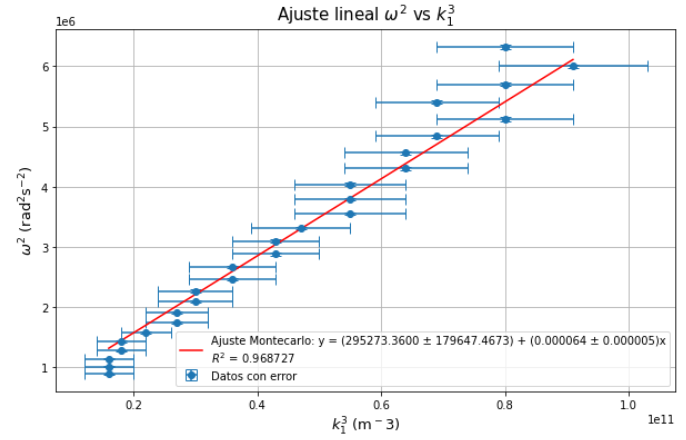
\includegraphics[width=\textwidth]{grafico_02x04_w2k13.png}
		\centering(a)
	\end{minipage}
	\hspace{0.5cm}
	\begin{minipage}{0.485\textwidth} 
		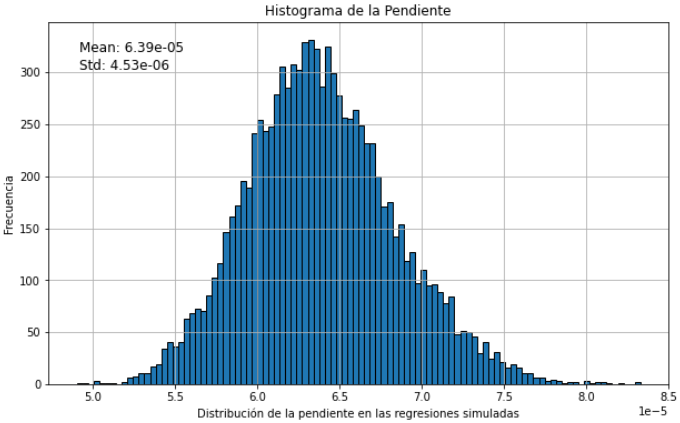
\includegraphics[width=1\textwidth]{grafico_02x05_w2k13hist.png}
		\centering (b)
	\end{minipage}
	\caption{ \footnotesize {a) Ajuste lineal de w2 y $k_1^3$  b) Histograma de las 10000 simulaciones de regresión realizadas.}}
	\label{fig:w2k1}
\end{figure}

\begin{figure}[H]
	\centering
	\begin{minipage}{0.47\textwidth} 
		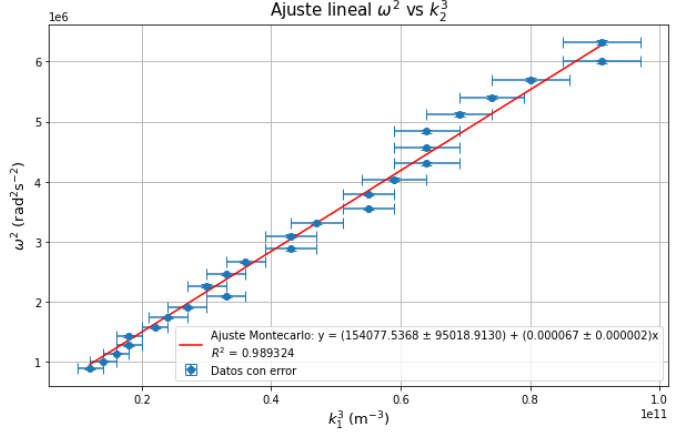
\includegraphics[width=\textwidth]{grafico_02x06_w2k23.png}
		\centering(a)
	\end{minipage}
	\hspace{0.5cm}
	\begin{minipage}{0.47\textwidth} 
		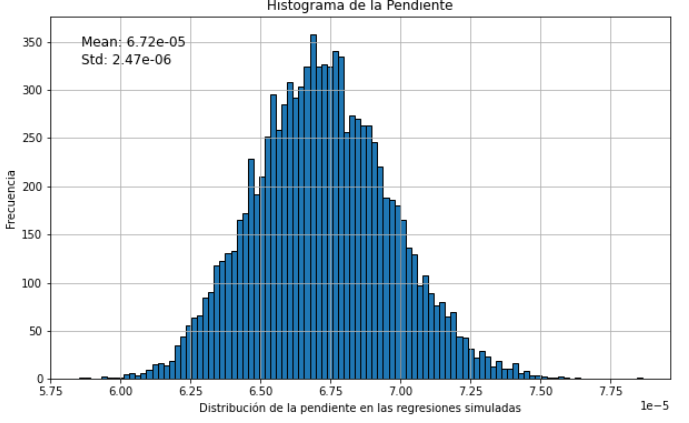
\includegraphics[width=1\textwidth]{grafico_02x07_w2k23hist.png}
		\centering (b)
	\end{minipage}
	\caption{ \footnotesize {a) Ajuste lineal de w2 y $k_2^3$  b) Histograma de las 10000 simulaciones de regresión realizadas.}}
	\label{fig:w2k1}
\end{figure}

\begin{figure}[H]
	\centering
	\begin{minipage}{0.46\textwidth} 
		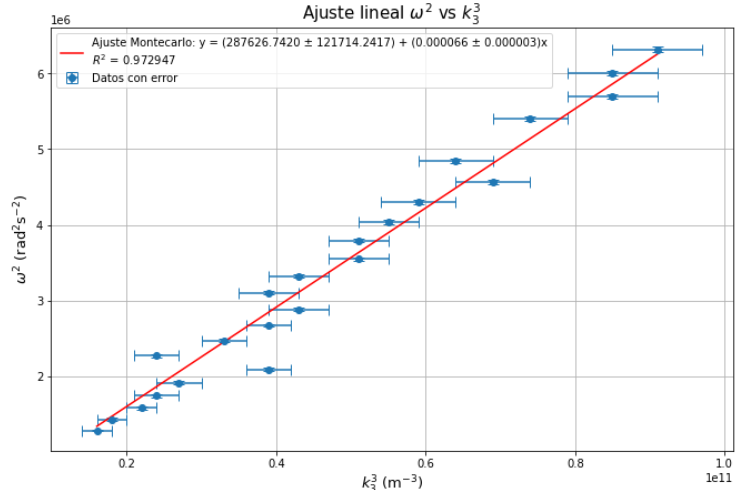
\includegraphics[width=\textwidth]{grafico_02x08_w2k33.png}
		\centering(a)
	\end{minipage}
	\hspace{0.5cm}
	\begin{minipage}{0.49\textwidth} 
		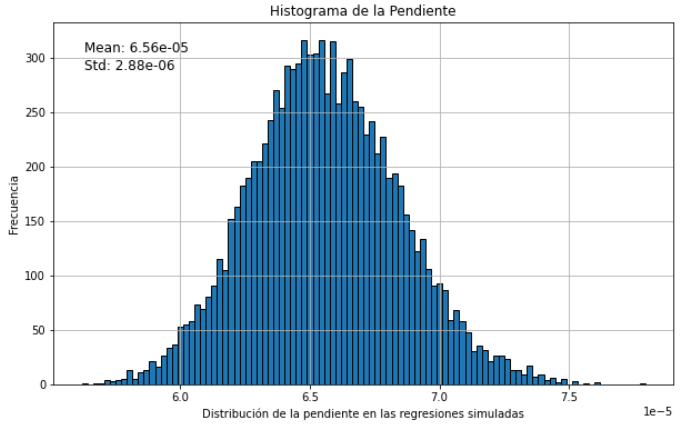
\includegraphics[width=1\textwidth]{grafico_02x09_w2k33hist.png}
		\centering (b)
	\end{minipage}
	\caption{ \footnotesize {a) Ajuste lineal de w2 y $k_3^3$  b) Histograma de las 10000 simulaciones de regresión realizadas.}}
	\label{fig:w2k1}
\end{figure}

\definecolor{gray}{rgb}{0.9,0.9,0.9} 
\begin{table}[H]
	\centering
	\begin{minipage}{0.7\textwidth} 
		\centering
		$\rho = 1000$ kg m$^{-3}$\\
		\begin{tabular}{|c|c|c|}
			\toprule
			n & $\alpha$ (m$^3$ s$^{-2}$) & $\sigma=\rho\alpha$ (N m$^{-1}$) \\
			\hline
			1 & (6.39$\pm$0.45$)\cdot$ 10$^{-5}$ & 0.0639$\pm$0.0045  \\
			2 & (6.72$\pm$0.25$)\cdot$ 10$^{-5}$ & 0.0672$\pm$0.0025  \\
			3 & (6.56$\pm$0.29$)\cdot$ 10$^{-5}$ & 0.0656$\pm$0.0029  \\
			\hline
			\cellcolor{gray} & \cellcolor{gray}  & \textbf{0.0656$\pm$0.0033}    \\
			\bottomrule
		\end{tabular}
		\caption{\footnotesize Estimación final de la tensión superficial del agua.}
		\label{tab:sigmas}
	\end{minipage}
\end{table}


Obtenidos los valores de las pendientes $\alpha_i$ para los tres casos, podemos hacer una estimación final de la tensión superficial $\sigma$ a partir de ellos promediando tanto las cantidades sus incertidumbres tal y como se indica en la tabla \ref{tab:sigmas}.

\vspace{\baselineskip}

Ahora bien, el valor promediado  es para $T=24\pm1$, es decir, $\sigma_{(T=24)} = 0.0656\pm0.0033$ N m$^{-1}$. El valor de referencia de acuerdo a CODATA \cite{Vargaftik1983} es $\sigma_{(T=25)} = 0.07599\pm0.0004$ N m$^{-1}$, que lo podemos tomar como aproximación válida. Nuestra estimación tiene un error relativo del 5\% lo que es una precisión aceptable.

\vspace{\baselineskip}

No obstante, la  nuestra estimación difiere del valor de referencia en aproximadamente 0.01039 N/m, lo que corresponde a una desviación de 3.13 veces la desviación estándar combinada \ref{eq:stdcomb}.

\vspace{\baselineskip}
\begin{equation}\label{eq:stdcomb}
	\Delta \sigma_\text{combinada}= \sqrt{(\Delta \sigma_\text{calculado})^2 + (\Delta \sigma_\text{referencia})^2} = 0.003342 \text{ N/m}
\end{equation}

\vspace{\baselineskip}
Esta desviación también representa un 13.67\% en términos porcentuales,  Además, al comparar los rangos de incertidumbre ([0.0623,0.0689] vs [0.07559,0.07639]), se observa que no hay solapamiento entre los intervalos de las dos medidas.







\section{Discusión}


De acuerdo  al estimaciones hechas de la tensión superficial \ref{tab:sigmas} para los diferentes ordenes de difracción, la proximidad entre los tres valores calculados sugiere una buena consistencia interna del metodología aplicada.

\vspace{\baselineskip}

No obstante, el comparar la estimación final con el valor de referencia para la tensión superficial del agua a 25°C hay una diferencia de  un 13.67\% en magnitud. Las causas para ello han podido residir en sesgos en nuestro método de medición o en la calibración del equipo. Además la estimación visual de las distancias  $c_i$ de los patrones de difracción sobre papel milimetrado esta sujeta a imprecisiones inherentes al observador y del ajuste adecuado del dispositivo experimental.

\vspace{\baselineskip}

Cabe señalar también que temperatura entre nuestro experimento (24 ± 1°C) y la temperatura de referencia (25°C) no puede explicar la discrepancia observada, ya que la variación de la tensión superficial del agua en este rango de temperatura es muy pequeña \cite{Vargaftik1983}.

\vspace{\baselineskip}

A pesar de la discrepancia con el valor de referencia, la alta linealidad observada en los gráficos de $\omega^2$ vs $k^3$  (R² > 0.96 para todos los órdenes) sugiere que el método es fundamentalmente sólido y que la relación de dispersión utilizada es apropiada para este rango de frecuencias.


\section{Conclusiones}

El experimento llevado a cabo logró estimar la tensión superficial del agua con un grado de precisión moderado. La consistencia interna entre los diferentes órdenes de difracción y la fuerte linealidad en los gráficos de $\omega^2$ vs $k^3$ respaldan la validez del método. Sin embargo, la discrepancia significativa con el valor de referencia sugiere la presencia de errores sistemáticos que requieren investigación adicional. Para futuros experimentos, se recomienda:

\begin{enumerate}
\item Investigar a fondo posibles fuentes de error sistemático en el montaje experimental y en el procesamiento de datos.
\item Utilizar agua de mayor pureza y verificar su calidad.
\item Realizar múltiples series de mediciones para evaluar mejor la reproducibilidad.
\item Dar mayor peso a las mediciones de segundo y tercer orden, que mostraron menor incertidumbre.
\end{enumerate}

La investigación de los errores sistemáticos debería ser la prioridad, dado que la variación por temperatura ha sido descartada como una fuente significativa de error.


\begin{thebibliography}{99}
	
	\bibitem{Jones1924}
	White, F. M. (2004). Mecánica de Fluidos (5ª ed.). McGraw-Hill.


	\bibitem{Anderson_montecarlo} Anderson, G. M., \textit{Error propagation by the Monte Carlo method in geochemical calculations}, Geochimica et Cosmochimica Acta, 40(12), 1533-1538, 1976

	\bibitem{error_prop} Bevington, Philip R., y D. Keith Robinson. \textit{Data Reduction and Error Analysis for the Physical Sciences}. 3ra ed., McGraw-Hill, 2003.
	
	\bibitem{Vargaftik1983}
	Vargaftik, N. B., et al. (1983). International Tables of the Surface Tension of Water. Journal of Physical and Chemical Reference Data, 12(3), 817. \url{https://doi.org/10.1063/1.555688}
	
	
	
	
\end{thebibliography}





    
   
\end{document}
